\section{Лекция 17.05.2018}

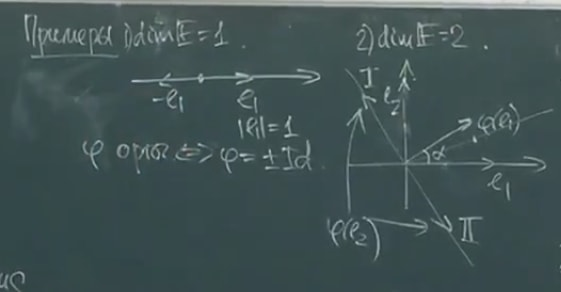
\includegraphics[width=15cm,height=12cm,keepaspectratio]{examples1.jpg}

\bigskip
$(e_1, e_2)$ -- ортонормированный базис

\bigskip
\RomanNumeralCaps{1} $A(\varphi, e) = \begin{pmatrix} \cos \alpha && -\sin \alpha \\ \sin \alpha && \cos \alpha
\end{pmatrix} \Rightarrow \varphi$ -- поворот на угол $\alpha$

\bigskip
\RomanNumeralCaps{2} $A(\varphi, e) = \begin{pmatrix} \cos \alpha && \sin \alpha \\ \sin \alpha && -\cos \alpha \end{pmatrix} \Rightarrow \varphi$ -- поворот на угол $\alpha$ + отражение относительно $\varphi(e_1)$

Пусть $l$ -- биссектриса угла $\angle (e_1, \varphi(e_1))$. Тогда $\forall \ v \in l: \varphi(v) = v, \forall \ v \in l^{\bot}: \varphi(v) = -v$

$e' = (e'_1, e'_2)$ -- ортонормированный базис, $e'_1 \in l, e'_2 \in l^{\bot} \Rightarrow A(\varphi, e') = \begin{pmatrix} 1 & 0 \\ 0 & -1 \end{pmatrix}$

$\Rightarrow \varphi$ -- отражение относительно $l$

\bigskip
\textbf{Предложение.} $\varphi$ -- ортогональный линейный оператор, $U \subseteq E$ -- $\varphi$-инвариантное подпространство $\Rightarrow U^{\bot}$ тоже $\varphi$-инвариантно

\bigskip
\textbf{\textit{Доказательство.}} $\rhd \ \psi := \varphi|_{U}$ -- ортогональный линейный оператор в $U \Rightarrow \exists \ \psi^{-1} = \psi^*$

Хотим: $\forall \ x \in U^{\bot} \ \forall \ y \in U: (\varphi(x), y) = 0$

$(\varphi(x), y) = (x, \varphi^*(y)) = (x, \varphi^{-1}(x)) = (\overbrace{x}^{\in U^{\bot}}, \overbrace{\psi^{-1}(y)}^{\in U}) = 0 \ \lhd$

\bigskip
\textbf{Теорема.} $\forall$ ортогонального линейного оператора $\varphi \in L(E) \ \exists$ ортонормированный базис $e$, такой что \begin{equation*}A(\varphi, e) = \left(
\begin{array}{c|c|c|c|c|c|c|c|c|c}
  П(\alpha_1) & 0 & 0 & 0 & 0 & 0 & 0 & 0 & 0 & 0  \\
  \hline
  0 & П(\alpha_2) & 0 & 0 & 0 & 0 & 0 & 0 & 0 & 0  \\
  \hline
  0 & 0 & \ddots & 0 & 0 & 0 & 0 & 0 & 0 & 0  \\
  \hline
  0 & 0 & 0 & П(\alpha_k) & 0 & 0 & 0 & 0 & 0 & 0 \\
  \hline
  0 & 0 & 0 & 0 & -1 & 0 & 0 & 0 & 0 & 0 \\
  \hline
  0 & 0 & 0 & 0 & 0 & \ddots & 0 & 0 & 0 & 0 \\
  \hline
  0 & 0 & 0 & 0 & 0 & 0 & -1 & 0 & 0 & 0 \\
  \hline
  0 & 0 & 0 & 0 & 0 & 0 & 0 & 1 & 0 & 0 \\
  \hline
  0 & 0 & 0 & 0 & 0 & 0 & 0 & 0 & \ddots & 0 \\
  \hline
  0 & 0 & 0 & 0 & 0 & 0 & 0 & 0 & 0 & 1 \\
\end{array}
\right) (*)\end{equation*}

$П(\alpha) = \begin{pmatrix} \cos \alpha && -\sin \alpha \\ \sin \alpha && \cos \alpha \end{pmatrix}$

\bigskip
\textbf{\textit{Доказательство.}} $\rhd$ Индукция по $n = dimE, n=1, 2 \Rightarrow$ было.

Пусть теперь $n \geqslant 3$.

$\exists \ \varphi$-инвариантное подпространство $U$, такое что $dimU = 1$ или $2 \Rightarrow$ в $U$ требуемый базис $\exists$

$U^{\bot}$ -- $\varphi$-инвариантно, $\varphi|_{U^{\bot}}$ -- ортогональный оператор

$dimU^{\bot} = n - dimU < n \Rightarrow$ по предположению индукции в $U^{\bot} \ \exists$ требуемый ортонормированный базис.

Объединяя полученные базисы для $U$ и $U^{\bot}$, получим ортонормированный базис $e$, такой что $A(\varphi, e)$ имеет вид $(*)$ с точностью до перестановки блоков $\lhd$

\bigskip
\textbf{Следствие.} $\forall$ ортогонального линейного оператора $\varphi$ в 3-мерном евклидовом пространстве $\exists$ ортонормированный базис $e$, такой что $A(\varphi, e)$ имеет один из следующих двух видов:

\RomanNumeralCaps{1} $\begin{pmatrix} П(\alpha) & 0 \\ 0 & 1 \end{pmatrix}$ -- поворот вокруг $<e_3>$ на угол $\alpha$

\RomanNumeralCaps{2} $\begin{pmatrix} П(\alpha) & 0 \\ 0 & -1 \end{pmatrix}$ -- поворот вокруг $<e_3>$ на угол $\alpha$ + отражение относительно $<e_1, e_2> = <e_3>^{\bot}$ = "зеркальный поворот"

\bigskip
\textbf{\textit{Доказательство.}} $\rhd$ По теореме $\exists$ ортонормированный базис $e$, такой что $A(\varphi, e)$ имеет вид $(*)$. Если в $(*)$ есть блок $П(\alpha)$, то ОК. Если нет, то $A(\varphi, e) = \begin{pmatrix} \pm 1 & 0 & 0 \\ 0 & \pm 1 & 0 \\ 0 & 0 & \pm 1 \end{pmatrix}$

$\begin{pmatrix} 1 & 0 \\ 0 & 1 \end{pmatrix} = П(0)$

$\begin{pmatrix} -1 & 0 \\ 0 & -1 \end{pmatrix} = П(\pi) \lhd$

\subsection{Сингулярное разложение}

\textbf{Напоминание}:

$V, W$ -- векторные пространства над $F$, $\varphi: V \rightarrow W$ -- линейное отображение, $dim V = n, dim W = m$, $rk \varphi = r \Rightarrow \exists$ базис $e$ в $V$ и базис $f$ в $W$ такие, что 

\begin{equation*} A(\varphi, e, f) = \bordermatrix{ 
    	 & & & r & & & & n \cr
    	 & 1 & \cdots & 0 & \dots & \cdots & \cdots & 0 \cr 
         & 0 & \ddots & 0 & \dots & \cdots & \cdots & 0 \cr
		r & 0 & \cdots & 1 & \dots & 0 & 0 & 0  \cr
         & \vdots & \vdots & \vdots & \vdots & \vdots & \vdots & \vdots \cr
        & 0 & 0 & 0 & \dots & 0 & 0 & 0  \cr
        & 0 & 0 & 0 & \dots & 0 & 0 & 0  \cr
       m & 0 & 0 & 0 & \dots  & 0 & 0 & 0 }, r = rk \varphi = dim Im \varphi
\end{equation*}

\bigskip
$E$ -- евклидово пространство со скалярным произведением $(\cdot, \cdot), dimE = n$

$E'$ -- евклидово пространство со скалярным произведением $(\cdot, \cdot)', dimE = m$

\bigskip
\textbf{Теорема о сингулярных базисах.} $\varphi: E \rightarrow E'$ -- линейное отображение, $r = rk \varphi \Rightarrow \exists$ ортонормированный базис $e$ в $E$ и ортонормированный базис $e'$ в $E'$, такой что \begin{equation*}A(\varphi, e, f) = \begin{pmatrix} \sigma_1 & 0 & 0 & 0 & 0 & 0 & 0 \\  0 & \sigma_2 & 0 & 0 & 0 & 0 & 0 \\ 0 & 0 & \ddots & 0 & 0 & 0 & 0 \\ 0 & 0 & 0 & \sigma_r & 0 & 0 & 0 \\ 0 & 0 & 0 & 0 & 0 & 0 & 0 \\ 0 & 0 & 0 & 0 & 0 & \ddots & 0 \\ 0 & 0 & 0 & 0 & 0 & 0 & 0  \end{pmatrix}\end{equation*}, где $\sigma_1 \geqslant \sigma_2 \geqslant \dots \geqslant \sigma_r > 0$

Более того, числа $\sigma_1, \dots, \sigma_r$ определены однозначно.

\bigskip
\textbf{\textit{Доказательство.}} $\rhd$ Рассмотрим сопряженный линейный оператор $\varphi^*: E' \rightarrow E$

$(\varphi(x), y)' = (x, \varphi^*(y)) \ \forall \ x \in E, y \in E'$

\bigskip
Положим $\psi:= \varphi^* \varphi, \psi \in L(E)$

$x, y \in E \ (\psi(x), y) = (\varphi^* \varphi(x), y) = (\varphi(x), \varphi(y))' \Rightarrow (\psi(x), y) = (x, \psi(y)) \Rightarrow \psi = \psi^*$

\bigskip
Для $\psi \ \exists$ ортонормированный базис $e = (e_1, \dots, e_n)$, такой что $A(\psi, e) = diag(s_1, \dots, s_n)$

\bigskip
$\forall \ i = 1, \dots, n: (\psi(e_i), e_i) = (\varphi(e_i), \varphi(e_i))' \geqslant 0$ и $(s_i e_i, e_i) = s_1 (e_i, e_i) = s_i \Rightarrow s_i \geqslant 0$

\bigskip
Переставив векторы в $e$ можем считать, что $s_1 \geqslant s_2 \geqslant \dots \geqslant s_n \geqslant 0$

\bigskip
Пусть $k$ таково, что $s_k \neq 0, s_{k+1} = 0$, тогда $\forall i \geqslant k + 1, 0 = s_i = (\varphi(e_i), \varphi(e_i))' \Rightarrow \varphi(e_i) = 0 \Rightarrow e_i \in Ker \varphi$

\bigskip
$\forall \ i = 1, \dots, k$ положим $\sigma_i = \sqrt[]{s_i}$ и $f_i = \frac{1}{\sigma_i} \varphi(e_i) \in E'$

$\forall \ i, j = 1, \dots, k$ имеем $(f_i, f_j)' = (\frac{1}{\sigma_i} \varphi(e_i), \frac{1}{\sigma_j} \varphi(e_j))' = \frac{1}{\sigma_i \sigma_j}(\varphi(e_i), \varphi(e_j))' = \frac{1}{\sigma_i \sigma_j}(e_i, \varphi^* \varphi(e_j))' = \frac{1}{\sigma_i \sigma_j}(e_i, \psi(e_j))' = \frac{1}{\sigma_i \sigma_j}(e_i, \sigma_j^2 e_j)' = \frac{\sigma_j}{\sigma_i} (e_i, e_j) = \frac{\sigma_j}{\sigma_i} \delta_{ij} = \delta_{ij}$

$\Rightarrow (f_1, \dots, f_k)$ -- ортонормированная система в $E'$

\bigskip
Дополним ее до ортонормированного базиса $f = (f_1, \dots, f_m)$ в $E'$

Тогда $A(\varphi, e, f) = \begin{pmatrix} \sigma_1 & 0 & 0 & 0 & 0 & 0 & 0 \\  0 & \sigma_2 & 0 & 0 & 0 & 0 & 0 \\ 0 & 0 & \ddots & 0 & 0 & 0 & 0 \\ 0 & 0 & 0 & \sigma_r & 0 & 0 & 0 \\ 0 & 0 & 0 & 0 & 0 & 0 & 0 \\ 0 & 0 & 0 & 0 & 0 & \ddots & 0 \\ 0 & 0 & 0 & 0 & 0 & 0 & 0  \end{pmatrix} \Rightarrow k = rk \varphi = r$

\bigskip
Числа $\sigma_1^2, \sigma_2^2, \dots, \sigma_r^2$ суть все ненулевые собственные значения линейного оператора $\psi = \varphi^* \varphi$ и потому определены однозначно $\lhd$

\bigskip
\textbf{Определение.} В условиях теоремы $e, f$ называются \textit{сингулярными базисами линейного оператора} $\varphi$, числа $\sigma_1, \dots, \sigma_r$ называются \textit{сингулярными значениями линейного оператора} $\varphi$.

\bigskip
\textbf{Замечание.} 1) Вообще говоря, $e$ и $f$ определены не однозначно, $(e, f)$ -- сингулярные базисы $\Rightarrow (-e, -f)$ -- тоже сингулярные базисы

2) Доказательство теоремы дает алгоритм нахождения сингулярных базисов и сингулярных значений для $\varphi$

3) $e, f$ -- собственные базисы для $\varphi, \sigma_1, \dots, \sigma_r$ -- сингулярные значения $\Rightarrow A(\varphi^*, f, e) = A(\varphi, e, f)^T \Rightarrow f, e$ -- сингулярные базисы для $\varphi^*, \sigma_1, \dots, \sigma_r$ -- сингулярные значения для $\varphi^*$

